\chapter{逝去之梦}

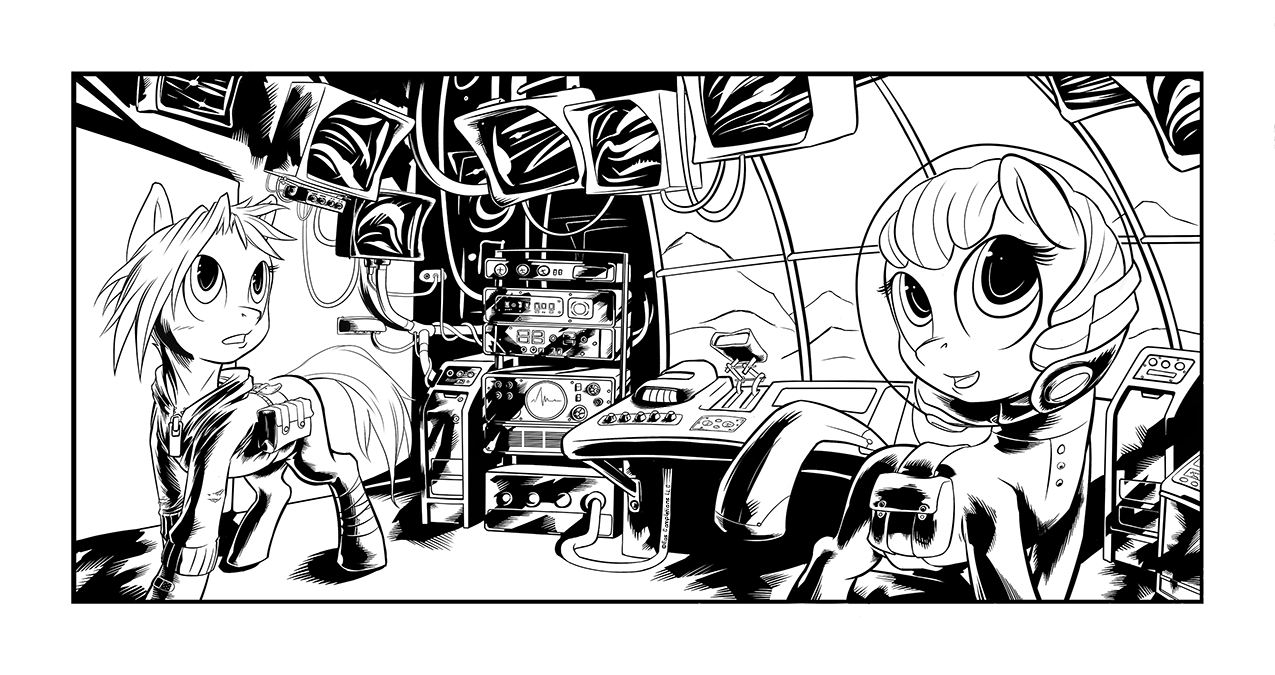
\includegraphics[width=0.9\linewidth]{image08.png}

\begin{intro}
那些床底下的黑影总让我担惊受怕。
\end{intro}

\daytimeplace{7}{3:00 AM}{旭日隧道,隧道镇}{Solaris Tunnel, Tunnel Town}

打了个哈欠,扳机低头看着幼驹在控制室地上玩。帕比正在一边用嘴发出『嘟嘟』声一边玩着一辆玩具车,她把一堆瓶盖放在车上,然后卸到一个闪闪可乐空瓶子边,然后再把瓶子装在车上。

「可以给我超级特别薄荷口味吗?好,谢谢,再见……」幼驹小声地玩着,好像她担心发出噪声惊扰到其他小马……

\thpr{她怎么做到的?把所有那些烦恼都丢在一边,然后就那样……坐下来玩儿?像个普通孩子一样?}

「喏,小家伙,你朋友怎么样了?」

帕比一边继续玩着她的玩具一边回答:「不知道,她说要花好一阵子呢,所以我要在这里等她……」现在幼驹似乎在用什么做一个围栏。

扳机吓了一跳,「你怎么还带着 9\,mm 子弹?」

「哦,那些啊?闪闪发光的漂漂东西,而且好像有个揪耗毛兽强啥的要用。」小雌驹埋头玩着玩具。

「啥啥啥?」

帕比伸起蹄子大喊着:「吵吵的东西!」一把破破烂烂的九毫米半自动手枪出现在她蹄子上,吓得扳机连忙躲到一台终端后面。

「喂喂,谁给你那玩意儿的?很危险的!」

「才不,这东西吵死了……我也不喜欢,只有小雄驹才喜欢这种玩具的啦,除非它是粉色的话……」

女卫兵紧张地笑着,「对哦,帕比,那东西一点都不好玩,想换点有趣儿的东西么?」

这句话引起了帕比极大的兴趣,幼驹转过头来,水汪汪的粉色双眸闪闪发光,满怀期待的看着扳机。

「当然啊!你有什么?」

「呃,一个墨镜\footnote{墨镜:带墨镜的卫兵……黑杰克躺枪}如何?」

「好耶,墨镜!等等……」帕比皱起眉头,「我戴着这破头盔,戴不了墨镜的。」

扳机以蹄覆面,「好吧,抱歉小家伙,我想什么呢。」独角兽回头在她的鞍带里面翻着,「那么这本九成新的《缰绳八卦》杂志如何?里面全是漂漂马照片,还有小蝶的!」

帕比走到卫兵身边,看着杂志,然后开心地一蹦老高,「我喜欢这个,里面全是漂漂马!我认识这个,她是萍琪派!还有瑞瑞!哦哦,云宝黛茜!我超超超喜欢云宝!她可以飞在天上嘣嘣嘣!等我长大了我要当她的新娘子!我喜欢这个画册,给我嘛给我嘛给我嘛!」

扳机举起蹄子掩着自己嘴角的窃笑,「我想我们可以成交了,不过你要把子弹也给我。」

「好好好好!哦哦哦!这个大的子弹你能换给我什么?」帕比问着,又掏出一发大号的坦克用尾翼稳定脱壳穿甲弹头。

独角兽雌驹叹了口气,事情越来越麻烦了。

\horizonline

\daytimeplace{7}{3:00 AM}{糖霜咖啡馆,隧道镇}{Sugartop Cafe, Tunnel Town}

昏暗的咖啡馆里面现在烟雾缭绕,和每天夜里的这个时候一样,完全是个颓废的地方。几个醉醺醺的小马东倒西歪地躺在那里,吸着来历不明的药品,一只狮鹫躲在房间的角落,还有一只戴着墨西哥帽子的小马在弹七弦琴。酒保正在用一块黑得看不出颜色的抹布「清理」着地板,但是坏枪根本都不在乎这些。

「再来一杯!」他摇摇晃晃地举起空杯子,用力吸着里面的蓝色吸管,但是却发出空荡荡的吱吱声。「我说,你聋了么?我说再来一杯!」他不停地晃着酒杯但是谁也不搭理他,真是失望。

这里的酒保,那只黑鬃的银色公马,坐在他旁边放下一瓶闪闪可乐,「我说大家伙,安静点,客人在楼上睡觉呢!」

「闭嘴!老黑!」坏枪嘟囔着,「赶紧给我倒点儿给力的玩意儿,我真不敢相信她居然甩了我!」

年轻的伙计叹了口气,把可乐瓶推到坏枪嘴边。「拜托老兄,别惦记她了,赶紧睡觉去,你可以睡我楼上的床,别喝了,一点用都没有。」

卫兵看着他兄弟的脸,但是却不想从桌子上抬起脑袋来。

「你知道这酒吧有一半是我的么?」

「对,但是你每次来就是和我抱怨你过得有多悲催。然后呢,处理顾客,打扫卫生,撵走不付钱的醉鬼……」黑帽子在桌子上敲着蹄子,「老实说你帮我做了哪样?话说你自己就是个不付钱的醉鬼好么?」

坏枪挥着蹄子像是赶苍蝇一样嘘着他的兄弟,「滚边儿去老黑,你的臭气都快把我熏昏过去了,给我点新鲜空气。」

「那你为啥不去城外走两圈,好像坐在这里就会空气好一样。」

「闭嘴,再给我倒杯性感天马,老黑……」坏枪举着空杯子,脸却扎在桌子上。「她怎么可以……」

终于黑帽子发火了,「拜托,老兄,我知道你在说谁!就是那个快乐扳机,这是我见过最烂的婊……」

砰!

坏枪看着他趴在地上的兄弟,「老黑,你还真说错了,呆这里鬼混让我感觉到……嗯……非常好,」公马说着往外走,「谢了老弟。」

\horizonline

\daytimeplace{7}{3:15 AM}{旭日隧道,隧道镇}{Solaris Tunnel, Tunnel Town}

「帕比,你还记得……小马国两百……呃……在你离开中心城之前,那里怎样?」

小雌驹皱着眉头,想要想出个答案来。「新鲜!」

「新鲜?」

「没错,妈咪好像是某种士兵,但是她其实不喜欢打仗,她很擅长修东西,所以不是很危险的时候她都带着我。我见过很多神奇的好地方,比如说一个天马机场,还有地底下的一个叫避难厩的大地洞,但是完全不知道那是什么……而且我还到过小马镇,还有其它很多地方……」幼驹很自豪地抬头挺胸说:「不过52号国道的小马们看起来好可怜,这里没有青山绿水,也没有漂漂房子,小马们也都很不开心的样子。」

扳机感觉到有什么东西哽在喉咙里面,「如果……如果你不想说的话……就别说了。」

帕比看着独角兽,有些奇怪地回答:「为什么不想?虽然这里不如其它地方漂亮,但是这里也有很多大姐姐一样善良的漂漂马……或许等我找到妈妈可以带你去看那些漂漂地方……真的!我不知道为什么你们喜欢住在这种灰扑扑的地方。」

「呃……当然可以……不过……你可以先和我说说小马镇么?」

「当然!那可是我见过最漂亮甜美的小镇!那可是萍琪派去中心城之前住的地方!妈咪因为要去做很重要的事情所以让我在那里呆了整整一个暑假!我在那里交了好多朋友!而且那里的山丘和树木颜色都非常漂漂。哦哦哦,还有一个叫旋转木马的地方!但是并不是真的旋转木马,只是名字……」帕比皱了皱眉头,「我只告诉你哦,因为那个时候我问为什么那里的木马都不转圈圈,大家都笑了,而妈妈也抱起我笑,不过我却觉得自己超级蠢……所以……别问我为什么木马不会转哦。」

扳机咯咯笑着点了点头:「别担心,我不会问的。」

「然后那里的苹果园中间还挖了一个超级大超级大的水洞。哦哦,那里还有一个城堡一样的云屋,上面还有彩虹瀑布落下来!对了,还有个商店卖羽毛笔和沙发!」帕比看着扳机的表情,担心地问:「乐乐姐我说错了什么吗?为什么你哭了?」

「我……我没哭,只是眼睛进了东西……」

「哈喽!都给我乐起来,小姐们!P7来啦!」忽然房间里面的所有屏幕都变成了粉色,每个屏幕上都出现了好像七个气球捆一起的标记。

「你好,声音小姐!谢谢你能过来!」帕比对着最大的屏幕挥着蹄子,那里的气球已经被一行字代替。

「多谢你给我找的新家,帕比!这里比那个到处漏风进雨的破圆顶好多了!我们看看这里有什么……哦!地热发电机!维护机器马离线……这个简单……哦哦!还有好多好多秘密文件还有……呃……红色安全警报?我怎么忘了这东西?」声音暂停了一会。

「有什么不对吗,声音小姐?」

「没,只是我需要旭日公司的某个大头头的授权来解除警告,不过好像已经有某小马在程序上开了后门,所以我可以简单地绕进去,一会儿就搞定!」

扳机有点狐疑地看着屏幕,她从来不喜欢A.I.,但是这个看起来很友善,帕比也认识她,所以她决定还是等等看发生了什么。

而帕比已经完全放松下来了。小雌驹和往常一样天真灿烂地笑着蹲坐在大屏幕面前,「好的好滴,你现在能找到我妈妈是不是在附近么?超超拜托?」

「红色警报解除!所有系统正常,安全门即将打开,5、4……哦,我不知道帕比,这里的主机是个巨大的数据库,而且没有授权的话我不能……哦哦等等……我在这里找到『那一天』之后三个星期的数据……不过我需要一个密码……」

小雌驹举起蹄子,「我知道!快乐帕比!」

扳机叹了口气,「帕比,你的名字不可能解开所有东西,你知道……」

「密码正确,虽然这东西都放了有两个世纪了,我把它们显示在大屏幕上。」

幼驹皱着眉头颠过来倒过去地把这几行字看了几遍,然后泪汪汪地转回头来。

「帮帮忙……」

独角兽雌驹坐在帕比身边,然后用蹄子轻轻搂着她的脖子,「当然小家伙,我读给你听好不好?」

\medskip

\begin{center}
\textbf{第十八天}
\end{center}

\wrpr{如果我还有向塞拉斯蒂娅公主祈祷的权力的话,我真希望避难所科技的那些书呆子来做这些工作,而不是旭日公司的这群}

\medskip

% NOTE: 译文错误

「呃,骡子,没错帕比,就是骡子……」

\medskip

\wrpr{这傻蛋旭日公司还真搞出一个在紧急状况下把优先权赋予技工的协议。但是这帮蠢货居然忘记给机器卫兵设置敌我识别!}

\medskip

「呃,这个词没啥意思,帕比,我们继续……」

\medskip

\wrpr{至少隧道现在还安全,我会在这里扎营几天,然后收集一下补给品为穿越沙漠做准备。}

\wrpr{已经快凌晨两点了,但是我睡不着,我好想她!我知道她在避难所里面很安全,但是我还能听到她因为怕黑和做恶梦拼命叫我的名字,但是我醒来却发现只是个噩梦。}

\medskip

「胡扯……嗯,是的,胡扯。」

\medskip

\wrpr{我应该给自己找点儿事干,免得我发疯,我恨小马国}

\medskip

「嗯,这部分是向女神的小小祈祷。」

\begin{flushright}
\textbf{阴雨·黛丝}
\end{flushright}

\medskip


扳机叹了口气,\wrpr{阴雨·黛丝女士写这个的时候,她绝对没想到她的小女儿真能读到这个东西}。

「好吧,看起来她继续往南走了……我们继续看看下面的记录。」

 P7打断她们的对话问道:「喂,帕比,你记得沙盒主任的密码么,超超拜托!」

幼驹戳着自己的头盔思考着。「玛塔莎?不对……是阿加莎!」

「谢谢啦,亲,我超超超想给你个大拥抱,让我们做做看吧,你先抱一下你自己,然后就当是我抱的好了!这里还有第二个文件,我会去我不该去看的地方转转看,你们好好玩儿,别弄得一团糟哦。」

\medskip

\begin{center}
\textbf{第二十一天}
\end{center}

\wrpr{我终于准备出发了,看起来没有其他小马来这个方向,我难道是这里唯一的幸存者?不太可能,但是我不想赌自己的运气,我打算绕开太阳城,这里被核弹头密集轰炸过,昨晚我都能在沙漠中看到那诡异的辐射光。如果我走运的话,几天之后我就能走到蓝羽机场了。我一天亮就出发。}

\wrpr{我还是睡不着,我一直梦见帕比死在厨房的地板上……}

\medskip

「胡扯,帕比,胡扯……」

「你喜欢胡扯么?」

「好了好了我继续读……」

\medskip

\wrpr{这只是噩梦,我很确信她很安全,她从来没有不听话过,为什么我一直梦到她?我找到一些药片,其中一些可以当安眠药,如果再做噩梦的话我就吃点儿。}

\begin{flushright}
\textbf{阴雨·黛丝}
\end{flushright}

\medskip


帕比紧紧地抱着卫兵,头盔紧紧压着扳机的后背。

「怎么了小家伙?她只是想你了,你现在好得很,等你找到她之后你就没事了,她也不会做噩梦了,对吧?」

和幼驹扯这种毫不羞耻的谎话让扳机的内心如同刀绞,但是帕比现在需要安慰。

「我……我不是好孩子,乐乐姐……我没有去那个秘密地方,因为我想去看烟花!」幼驹大哭起来,「我是坏孩子,妈妈会生我气的!」

扳机转身抱起小雌驹,安慰着她,「好了好了,别担心,你妈妈说了她要往南走,对吧?去一个……什么蓝羽机场?……我想那里就是铁锈庄园了,去那里很简单,只要绕过太阳城就到了,她再见到你一定很开心的!」

\thpr{为什么我要给这个可怜的小家伙希望?她妈妈早已经死了,我到底在做什么啊!}

那双清澈的粉红双眸中燃起了新的希望,帕比凝望着雌驹,「真的?她会在那里吗?」

「我……我也不知道她是不是,不过你想要追上她吧,对吧?如果你想要寻求真相,你必须跟着她新的足迹继续前进!」\thpr{没错,乐乐,两百年前的新足迹。}

幼驹又一次笑了起来:「对!我去什么地方都没关系,跟着妈妈,我去什么地方都可以!谢谢你乐乐姐姐!你是最棒的小马!」

 P7又一次打断了她们,「非常好,我搞定这里的物品清单了,好像旭日公司的家伙早就开始为『小马国末日』做准备了,这里有好多实验室,而且还有足够的军火再给那些幸存者来一次烟火秀!哦哦,帕比,我想你刚才又把萍琪派的名字给念错了!」

帕比抬起了头,「啥米?」

「简单的说,朋友,在这个山下面有好多好多层仓库,装满了各种军火,那些东西足够把小马国上的每一个混蛋都杀死两次!」

「呃……你说『杀死』是说,伤的很重?」小雌驹狐疑着问。

「不对不对!我是说伤得超级重!就像一个所有小马进去以后就出不来的超级大派对!」

「一个……机器萍琪派对?」帕比不由得打了个寒战,完全不想听到之后的回答。

「机械萍琪:文件未找到。」

帕比想了想然后又问:「好了,那么这些东西有些什么呢?」

「我们举几个例子吧!比如说『长程多弹头电浆导弹』这玩意能分裂成56个弹头同时命中56个不同的目标,每个弹头都可以轻易击穿地下防御掩体,然后把整个密闭空间灌满电浆,把温度瞬间上升到几千度,杀死里面的所有小马!还有『广域解离射线发生器』,可以把一百米之内的所有目标分解成原子状态,当然也会杀死小马。哦哦,还有『巧克力混沌\footnote{巧克力混沌(Chocolate chaos):正剧 S02E01,无序躺枪}』这个魔能武器可以把目标的血液变成巧克力牛奶!虽然效果会在一个半小时后消失,不过被打中的马当然也是立刻就死翘翘啦!」

「好了好了,不用说了……」帕比打断她的话。

「那么,我们该怎么办?你是老大!」

电脑最后一句话的话音刚落,扳机连忙举起蹄子想阻止小雌驹说出任何蠢话,不过她还是不够快。

「把它们全扔了!挖个大洞把那些东西都丢进去,在上面盖个房子然后把这里的所有坏蛋机器都送进去,这样就不会有小马受伤了!」

「好吧,从技术上讲,所有东西已经在这个山下面的大洞里面了……我可以炸毁通向仓库的电梯,除非有谁把整个山都挖开,否则他们肯定找不到那些东西了。」

「就这么办!」

扳机松了长长一口气。

\horizonline

\daytimeplace{7}{3:30 AM}{隧道镇,52号国道北口}{Tunnel Town, Big 52 N Branch}

坏枪用头撞着隧道的大铁门。

「肏,肏,我应该阻止她的……肏,肏,肏肏肏!」

「我说,老哥,就算你用力踢它,门也不会奇迹般地被你踢开的。」黑帽子坐在卫兵身边揉着眼睛,「我想这个乌眼青是我自找的,不过……这不代表我哪天会打回来。」

「看在露娜的份上,老黑!拿个腌青鱼压着那眼睛睡觉去,让我自己静一静行不行!」

银色公马靠在墙上打着哈欠,「没门儿,我才不会把我兄弟丢在这里,而且,这件事足够我笑话你几个月了。」

坏枪怒气冲冲地喷着响鼻,「我总怀疑我们老妈是个婊子,现在我很确定了,乐乐都已经不在了你还想笑!你是想再多个黑眼圈还是现在就滚蛋?」

「冷静点吧,你现在啥也做不了,这东西封得……我勒个去!」

一阵尖锐的金属摩擦声之后,大门缓缓升起,让黑帽子一屁股坐在了地上。

「我勒个大去……」

俩小马一脸难以置信的表情看着巨大的钢铁怪物——两米厚的巨大防水板慢慢升起,然后后面的另一扇隔板也缓缓让开。

坏枪傻站了快一分钟才张开嘴。「这……我……没做梦吧?掐我一下……」

砰!

「你这个尸鬼养的……我是说掐一下!」

老黑窃笑,「我说了你欠我一下,你还说她已经死了?」

两只雄驹蹄下跨过骷髅走进山洞内,黑帽子看着满是子弹孔的马车,又看着里面装的东西。「哇哦!这么多好东西!这小镇要发财了!」

坏枪则稍微走得远了一点,看着隧道的灯一盏一盏点亮,开始照亮这六公里长的地下隧道,而天花板上的一处通风道还挂着一根绳子,于是他撒开蹄子飞奔向山洞深处。

「等等老哥!别跑那么快!我们要叫上其他卫兵!」

「去你妹的卫兵!我喝高了而且还恋爱了!」雄驹的声音回荡在隧道中。

黑帽子叹了口气,跟着一起追了过去,「至少你等等我呀!」

\horizonline

\daytimeplace{7}{9:00 AM}{隧道南贸易站,52号国道中段}{Trade Station Tunnel South, Big 52 SC Branch}

扳机抱着帕比亲着她的头盔,而后者一脸不耐烦地拼命挣扎着。「唔……好肉麻,别在那么多小马面前亲亲!」

所有城镇卫兵和隧道镇的许多其他居民都围住了他们。在扳机护送着帕比走出隧道南口的时候,一位代表小镇政府的雌驹发表了一个小演讲,并且送给帕比一袋子瓶盖。

在两只小马面前是无边的地平线无数的沙丘,偶尔有几个红色的山石出现在视野中。在远处能够清晰地看到一个城市的剪影,但是沙漠的风尘让大家难以辨识这是真实的景象还是海市蜃楼。

「帕比,我们到了,这就是蛇蝎沙漠,你好好听我说怎么去铁锈庄园。」

小雌驹乐得蹦蹦跳跳的,「没问题,漂漂乐乐姐!」

「很好,这个荒漠是清砂工的领土,他们大多都是住在各种各样帐篷的拾荒者,在沙丘下面寻找各种有用的东西,不过我还是要提醒你,他们有时候还会抢劫,尤其是对于独行的旅者,但我觉得他们恐怕没那个胆子敢抢劫你,毕竟清砂帮是个非常迷信的氏族,而且他们肯定从孤狼那里听说过你的事了。」

帕比点了点头,「喜欢走来走去的漂漂马,懂了!」

扳机笑了笑,「很好,你只要跟着路标,很简单的,因为每隔50米清砂工就会放一面红色旗帜,你只要跟着旗子走,就能在明天早上之前到达他们的第一个营地。」

帕比皱着眉头指着旁边坚实的柏油马路,「为什么不走大路?踩着我的滑板在路上就像飞梭一般!」

「不行!小家伙,这个公路是直接通往太阳城的,你绝对不能去那个地方!」

「为啥?」

「那里是个危险的地方,所有小马去那里就再也没回来过!」扳机的声音中带着不容置疑的口吻,但是帕比完全没有在意。

她敲着自己头盔下巴的位置,「呃,或许他们超喜欢那里,所以不想走了呢?」

「我……我可不觉得……帕比,当我还是你这样的孩子时,太阳城是另一个氏族的地盘——锈刃,他们和清砂工是同盟……那是很久之前的事情了,但是后来听说清砂工找到了什么大家伙,而锈刃偷走了,然后就是说谁背叛谁的,最后他们就打起来了。最终清砂工想要策划一次突袭,在晚上夜袭城市。」雌驹顿了顿,看看幼驹还有没有在听。

「然后呢?」小听众有些担心地问。

「在突袭中发生了什么灾难,但是谁也不知道究竟出了什么事,只知道清砂工带了他们的所有武器冲进城市,但是却谁也没有回来,所有想要调查城市的小马都消失了,然后清砂工把剩下的小马聚集起来——大多都是老马和孩子,现在还在沙漠中挣扎求生。」

「所以,他们都是大坏蛋?」

班级皱了皱眉头,「在废土可没有什么明显的善恶之分,帕比,如果你想活下去,有些时候你必须做出一些……牺牲……就算是心碎也好,总比彻底失去生命要好。」

「呃……啥?」幼驹一脸茫然地看着扳机,不知道她话语之中的哲理。

「好了,别瞎想了小家伙,你就觉得……好吧……他们是坏蛋,但是他们不是自愿的。」

帕比摇了摇头,「不对!如果你做坏事,那你就是坏蛋!没有借口,如果觉得小小坏事就不算是坏事,那你最后就会做出大坏事,变成一个超级……超级大坏蛋!」

「呃……你自己想出来的么?」独角兽钦佩地看着帕比。

「才不是咧!妈妈说的!」

扳机拍拍帕比的头,看着她担心的表情,「别担心,打烂机器马不算坏事,妈妈不会不开心……好啦,笑一个!」

黄色的幼驹开心地跳上滑板车,「我见到妈妈以后会告诉她你对我超级好!谢谢你漂漂乐乐姐姐!」骑着滑板车,幼驹顺着沙漠的公路绝尘而去。

「呀呵呵……」

扳机看着幼驹骑着滑板越来越远,然后叹了口气,「我很抱歉,小家伙。」

「那么,乐乐,那就是那个小幽灵?」坏枪走到雌驹身边笑着问。

「我不知道,」扳机叹了口气,「我只知道她是个迷路的孩子。」然后她转头看着公马笑了起来,「你那熊猫眼哪里来的?」

「兄弟情谊纪念。」坏枪哼了一声,然后又说:「我们何曾不是迷失在这个残酷的世界之中呢?不过我想新闻一发出去的话,很快就会有大批小马来隧道镇了,我们要增招卫兵。」

「说到那个……马车上的货物应该回收,那些东西应该平分给每个小马,你帮我看好黑帽子。」

公马点了点头,「没错,别担心,其他小马已经把车拉回城了,有些车还是有标志的,有三个属于水头,还有一个是旋转木马的,不过上面的东西已经被和机器卫兵对干的小马糟蹋得差不多了。我们还给他们吗?」

「我们应该还给他们,至少作为我们善意的象征,他们知道我们帮他们保管好货物的话,也会乐于和我们合作的。哦,顺便提醒了我要教教你如果通道再次关闭的话该怎么打开。」

坏枪迟疑了一会之后又追问道:「还有,那个……昨晚那个……你知道的……在你追那个幽……帕比之后,我和你说了些……然后我们……能假装……我们什么也没说么……你知道的……那个……啥……」

扳机咯咯笑起来,「我可不觉得,大情圣……那可是我见过最笨的告白了,为了那些话,我也要和你过下半辈子啦。」

坏枪低下了头,「呃……我可以问问为什么吗?」

「我可以先问你一个问题么?」

公马挥着蹄子,「当然……问吧……把爱心之箭射入我心房吧……」

「我还有机会说……我也爱你吗?」

\horizonline

\daytimeplace{7}{4:00 PM}{蛇蝎沙漠,52号国道中段}{Serpent Desert, Big 52 SC Branch}

{\rt 女士们,先生们!下午好!这里是孤狼的52电台!小马国这片区域最好也是唯一的电台!昨天我正在街上走然后有小马问我,为什么大家都听你的节目?你的节目怎么会这么好?好吧,我必须承认那个不简单,因为我可是这附近唯一一个肏蛋DJ了。}

喇叭里一个女性在远处说:「{\rt 耶!!没错!}」

{\rt 坏孤狼,你说脏话了!你不应该说脏话的!尤其是我们的小英雄还在听你的节目的时候,对吧,对吧!我是个坏蛋我应该害臊才对。不过现在我却觉得很高兴,不,是非常高兴!因为一个带翅膀的朋友刚给我从南边带来了大新闻!做好心理准备,听众们,因为这个新闻超级劲爆!}

忽然随着一阵静电干扰声,广播中断了几秒钟,但是马上就恢复了。

「{\rt 好了,听众们我又回来了!你们竖起耳朵听好!谁也关不掉52电台,特别是今天,因为今天我们要一起庆祝隧道重新开张!没错小马们!你们耳朵没撒谎!隧道镇又回来了!再也不用走山路了!}」

狂野的音乐持续了一分多钟,而DJ在背景里面用嘴模仿着吉他的声音。

「{\rt 这可是砸烂嘉年华之后最大的好消息,猜猜是谁干的?没错,我们的守护天使!我们的小小幽灵!我们需要一个小孩子把我们从濒临饥荒之中拯救出来吗!肏你妈我太失望了!不过不开玩笑,一个小孩子,一个星期不到的时间,就把三个城镇从他们最恐怖的噩梦之中拯救出来了!一个小孩子而已!我说52,你们的骨气都哪儿去了?给我看看你们的信念!别让我一直崇拜一个比我小好多好多的小孩子行不行?}」

一阵沉寂之后,DJ的声音又回来了,这一次显得疲惫不堪。

「{\rt 醒醒吧伙计们,她只是一个孩子而已,她不可能搭救所有的小马,我们应该振作起来,我们自己就可以做得更好,我们不需要另一个英雄来崇拜!}」

一段悠扬的吉他声之后,另一段音乐响起,不过这次不是录音,而是孤狼自己唱的歌。

\begin{music}
走出废墟,走出残骸

\begin{englishlyric}
    Out of the ruins, out from the wreckage
\end{englishlyric}

\medskip

我们不能再犯同样的错误

\begin{englishlyric}
    Can't make the same mistake this time.
\end{englishlyric}

\medskip

我们是新一代的子女

\begin{englishlyric}
    We are the children, last generation.
\end{englishlyric}

\medskip

我们是被遗忘的一代

\begin{englishlyric}
    We are the ones they left behind\dots
\end{englishlyric}

\medskip

我们要改变这个时代

\begin{englishlyric}
    And I wonder when we are ever gonna change it,
\end{englishlyric}

\medskip

在恐惧和余烬之中挣扎求生我们一无所有

\begin{englishlyric}
    Living under the fear till nothing else remains.
\end{englishlyric}

\medskip

但是我们不需要更多英雄

\begin{englishlyric}
    We don't need another hero\dots
\end{englishlyric}
\end{music}

\horizonline

「哇哦,我真想见见他们说的那个超级英雄小雌驹!你觉得我们可以做朋友吗?」帕比跟着红色旗子在沙漠上走着。

「{\mtzh 肯定,通常英雄偶像都是相当友善的。警告,检测到中等辐射,威胁等级:可忽略。}」

幼驹一边走着一边问着:「对了,声音先生,你觉得我是好孩子吗,我妈妈还喜欢我吗?」

「{\mtzh 警告,该程序没有社交功能。}」

帕比长叹一声,「老天,每次问到关键问题你就躲起来,是吧?」她正想在说点什么,但是她的注意力被远处一个影子吸引了,「看,有个漂漂马!」

这个「漂漂」马看起来是一只鬃毛花白的红色独角兽,一件宽大的披风遮盖住了她的全身。当小雌驹走近的时候,她笑了,「慢慢来,小幽灵,我在中午就在这里等你了。」

「嗨,我是快乐帕比!」小雌驹挥着蹄子笑着说:「我很抱歉我迟……呃,我哪里迟到了?」

老马的嘴角微微挑起,「当然是探险……你喜欢探险吗?」

「是啊!我超超超爱探险!哪里可以探险?我能来两个吗?」忽然幼驹的表情变得严肃起来,「不对……等等……我还要找妈妈,不应该去探险……」

老马笑了笑,「没错,你已经有自己的路要走……我怎么忘了这个。」

帕比点了点头,「没错,我很抱歉,我该走了,谢谢,拜拜!」

「不过,如果我说这次探险是关于你的一个陷入危险的朋友呢?」

已经走开的幼驹又回过了头,「我的一个朋友?谁啊,为什么,在哪儿,什么时候?」

「好了,别急……」

帕比跳上长者的后背,用她的头盔贴上了她的鼻尖,她紧盯着独角兽的眼睛。

「拜托拜托快跟我说!」

老独角兽一下子没站稳,差点摔倒,「冷静一下,小幽灵,我正打算和你……快坐下听……好不好?乖乖的我就和你说话!」

「呃……好的……很抱歉漂漂老奶奶……」帕比放开她的脖子然后坐在独角兽面前,而后者松了一口气。

「我是先知长耳,一个可以看到远处景象的小马。」

帕比蹦蹦跳跳地说:「哦哦哦,你能看到我妈妈么?她能看到我们吗?她还好么?」

「不是那样的。」

小雌驹一瞬间泄了气坐了回去。

「我吃一些药之后,我可以在梦中看到一些景象,但是我不能选择我要看什么,昨晚我看见的是关于你的梦境。」

帕比安静地坐下来,在沙漠当中听着长耳慢慢讲故事。

「你让一个非常重要的朋友为你做一件很重要的事情,你的朋友竭尽全力,但是发生了一件非常糟糕的坏事,她没法再继续她的任务了,所以她在我的梦中让我来转告你。」

帕比皱了皱眉头,一个很重要的朋友帮一个大大的忙?但是她从来没有——哦哦,是丝尾!她让它照顾赫瑞别让坏事发生在她身上!

「赫瑞?她有危险?在哪里?」

雌驹点了点头,用蹄子指着远处的太阳城,「我恐怕那只小鹰飞得太靠近太阳,所以找不到回来的路了。」

帕比犹豫了一会,「但是……乐乐姐告诉我不能去那里!我要听她的话!」

长耳耸了耸肩,「你并不是非去不可,你让朋友帮忙,而她让我警告你,就是这样,你可以选择不管她,然后继续你的旅程。而我的任务也就是这样。」

「但是……但是有什么坏事发生在赫瑞身上!我不能把她丢下!她可能会受伤!她可能会哭!」

「那么,去太阳城救她吧,但是我要警告你,太阳城是一个陷阱,是个真实的噩梦,当你开始做梦之后,你就不能再离开了。」

「这个别担心,我一点都不困!」帕比笑得别提有多轻松了,「太空战士安德洛队长前去营救啦!」幼驹向城市奔去。

长耳看着飞奔的黄色幼驹,直到她远到化成一个灰色的小点儿,然后拿出一个药片,就着一瓶奶白色的液体吞了下去。但是老马能看到的只是火焰和枪声,

「我看到的是什么?过去还是未来?」

咯咯笑的声音在老马耳畔响起,「她很精神,一直在笑,我喜欢她!如果大家都能像她这样,不是一直板着脸的话……」

母马低语着:「但是一个梦魇能带来和平么?我不确定……」

「别问我啦!我只是你的迷幻剂带来的一个幻觉而已!真的,我帮不了你什么!就算你不看它,事情也会发生,而且你也不知道这个是过去还是未来。」

老独角兽叹了口气,「或许你是对的……我们回家吧。」

「对,我们走吧,帕比会照顾好自己的!」

~\vfill

\begin{note}
升级(Lv 7)

新技能解锁:钢铁力量——有时候光是石头还不够,你使用的所有钝击武器都增加5点额外伤害(没错,石头和动力蹄都属于钝击武器)。

任务技能:52之魂——你的传说在52号国道上流传,只要大多数氏族和你的关系保持中立或者中立以上,你随机遇到的低级敌对目标就会减少。
\end{note}

